\documentclass[conference]{IEEEtran}
\IEEEoverridecommandlockouts
\usepackage{cite}
\usepackage{amsmath,amssymb,amsfonts}
\usepackage{algorithmic}
\usepackage{graphicx}
\usepackage{subcaption}
\usepackage{textcomp}
\usepackage{xcolor}
\usepackage{xurl}
\usepackage[colorlinks=true,
            linkcolor=blue,
            citecolor=blue,
            urlcolor=blue,
            bookmarks=true]{hyperref}
\captionsetup[subfigure]{labelformat=parens,labelsep=space}
\def\BibTeX{{\rm B\kern-.05em{\sc i\kern-.025em b}\kern-.08em
    T\kern-.1667em\lower.7ex\hbox{E}\kern-.125emX}}


\usepackage{amsmath}
\usepackage{cuted}
\usepackage{stfloats}
\allowdisplaybreaks

\begin{document}

\title{A Simulation-Based Charging Station Recommendation Framework for
Electric Vehicles in Khulna City Using SUMO and TraCI}

\author{
\IEEEauthorblockN{Rakesh Biswas, Monishanker Halder, Md. Mahmudul Amin Shakil}
\IEEEauthorblockA{\textit{Department of Computer Science \& Engineering}\\
\textit{Jashore University of Science and Technology (JUST)}\\
Jashore, Bangladesh\\
200112.cse@student.just.edu.bd, m.halder@just.edu.bd, 200106.cse@student.just.edu.bd}
}

\maketitle

%-------------------------------------------------------
\begin{abstract}
The rapid growth of three wheeler electric vehicles -- Easy Bikes,
Electric-Rickshaws and Electric-Vans -all over the 
Bangladesh has great impact of unsupported charging demand on the urban
power infrastructure. It isn't prepared for a peak classification. Lack
of intelligent charging management systems reduces charging station
utilization efficiency, increases traffic congestion and the risk of
local power imbalance. To address those challenges, the paper represents
a simulation-based Electric Vehicle charging station recommendation
framework. It is developed using Eclipse SUMO microscopic traffic
simulator, which is integrated with Python and TraCI. With different
Electric Vehicle flows operating on multiple routes, a realistic urban
mobility scenario was created. The scenario is supported by
both-directional charging stations with realistic battery
specifications. The suggested recommendation engine continuously
observes -vehicles SoC, travel distance, slot-occupancy. Along with
monitoring instant electricity load, the proposed framework applies
multi valued decision model. With intelligent station selection enabled,
recommendations are made periodically in an advisory decision-making
mode to preserve traffic stability. Experimental results present that
proposed framework gains a potential recommendation rate of 90.1\%,
which exceeds the nearest only baseline(66\%). It also demonstrates
effective congestion avoidance capabilities. The simulation recorded a
peak charging demand of 1.37 MW with 40 simultaneously charging
vehicles. This reflects realistic urban load stress scenarios. The
resulting dataset supports machine learning based Electric Vehicle load
forecasting and smart grid planning studies \cite{b8} within the emerging Electric
Vehicle ecosystem.
\end{abstract}

\begin{IEEEkeywords}
Electric Vehicles, Easy Bike, E-Rickshaw, Charging Recommendation,
SUMO, TraCI, Smart Grid, Load Balancing, Bangladesh
\end{IEEEkeywords}

%=======================================================
\section{Introduction}
%=======================================================

The global adoption of electric vehicles (EVs) has accelerated as a
strategy to prevent greenhouse gas (GHG) emissions from the
transportation sector, which is responsible for approximately 38\% of
total global GHG production \cite{b1}. In Bangladesh, this change has
taken an individual form: instead of personal passenger cars,
battery-powered three-wheeled vehicles -- locally known as Easy Bikes
and E-Rickshaws -- have become the main intercity transportation medium \cite{b9}.

Khulna, the third largest city in Bangladesh and an important industrial
hub, is a case in point. Thousands of electric three-wheelers ply the
streets of Khulna every day, providing affordable, low-emission urban
mobility and supporting the livelihoods of a significant driver
population \cite{b2}. According to Khulna's traffic department, there are 30,000+ battery-driven easy bikes in the city, with Khulna City Corporation (KCC) having licensed 8,000 and processing approvals for another 2,000 \cite{b2}.

In spite of these facilities, EV charging in Khulna remains almost
completely imbalanced. Drivers select charging stations based only on
proximity and familiarity, which results in intense demand at popular
stations during morning and evening rush hours. Transformers serving to
those overloaded nodes - experience thermal stress, voltage drops, and
failures. This results repair costs and disruption of driver service \cite{b14}. In
the meantime peripheral stations remain continuously unused, which
highlights the infrastructure investment. Electric Vehicle load on the
electricity grid is projected to reach 780 TWh by 2030 \cite{b3, b4}
globally. It makes intelligent charging coordination an urgent
operational priority \cite{b16}.

Previous work on EV charging management has mainly addressed
advanced-economic contexts where vehicles are freely routable \cite{b5, b6} and have
the advantage of inter-vehicle navigation. There are 2 limitations in
the context of Khulna city which are absent in this literature : (i)
Easy Bikes and Electric Rickshaws and Electric Vans follow specific
corridor routes, as SUMO - the simulator used enforces one-way lane
assignment; (ii) charging infrastructure is scattered and heterogeneous
in terms of capacity, power rating and geographical distribution \cite{b15}. This
is a purpose-built simulation framework that realistically models the
Khulna fleet and designs around it rather than ignoring routing
limitations.

The paper represents a SUMO+TraCI simulation framework that models a
heterogeneous fleet of continuous 100 vehicles(Easy Bikes, Electric
Rickshaws, Electric Vans) on 8 road-routes \cite{b10, b11}. It monitors real time
battery SOC and also issues per vehicle charging station recommendations
through a multi criteria scoring models. This framework distinguishes
between potential routing -- when a directed network path exists. It
also suggests only output when directional limitations prevent routing.
In comparison with nearest only baseline, significant improvements are
seen in potential recommendation rates, congestion avoidance and genius
handling of high priority charging events. The contributions of this
work are: (i) a calibrated SUMO simulation of Khulna city's
heterogeneous Electric Vehicle fleet with physics-based battery modeling
on 3 vehicle classes; (ii) a multi-criteria recommendation algorithm
that clearly maintains SUMO directed routing; (iii) comparative
evaluation with nearest only baseline using four performance metrics;
(iv) a 33,721 recorded vehicle centric dataset.

%=======================================================
\section{Related Work}
%=======================================================

Planning of EV charging management research infrastructure, expands
real time routing, timesteps. We study every thread to indicate our
work position.

\subsection{Infrastructure Planning and Site Selection}

Wang et al. \cite{b2, b5} formulated charging station selection as a
multi-objective optimization problem. It reduces travel time, grid
pressure and cost through integer programming. Hussain et al. \cite{b6}
applied analytical classification. It was Analytic Hierarchy
Process(AHP). The methods combined with TOPSIS to rank candidate
stations according to accessibility, demand density, and grid capacity.
These methods inform long-term major decisions but do not indicate
real-time dispatch across existing networks. Rahman et al. \cite{b1}
surveyed adoption trends specific to Bangladesh, identifying
coordination gaps, which are directly correlated to this study. The study has also been conducted on the socio-economic and environmental impacts of battery-powered auto-rickshaws in Khulna city in accordance of Bangladeshi urban areas \cite{b15}. It is estimated that autorickshaws consume about 4,660 megawatt hours of electricity per day in Bangladesh \cite{b13}.

\subsection{Real-Time Routing and AI-Based Selection}

Current research explored reinforcement learning \& AI based frameworks
for dynamics Electric Vehicle charging distribution. These methods \cite{b7, b17}.
target to balance the load at stations, to lessen traffic, decrease
peak-demand through adaptive routing suggestion \cite{b12}. Microscopic traffic
simulation platforms like-SUMO has been widely implemented for traffic
optimization. More implementation for signal control, energy aware
mobility modeling \cite{b10, b19}. GIS-based multi-criteria decision-making approach for locating EV charging stations has also been demonstrated \cite{b18} By the way fixed work aggregated real time suggestive
recommendation of charging in to the heterogeneous EV fleet of South
Asian cities.

\subsection{Load Forecasting and Dataset Generation}

Siddiqui et al. \cite{b8} suggested DeepBoost---a stacked ensemble of
LSTM, XGBoost, CatBoost, and Linear Regression for day ahead EV
charging station load forecasting. It improved the MAE by 9.4\% and
32.7\%, respectively, compared to individual CatBoost and XGBoost on
the ACN dataset. Their work establishes - enriched feature engineering
-- station occupancy, depth of queue, SoC distribution, time of day.
The work drives forecast accuracy. The dataset produced by our
simulation accurately captures these features, making it directly
usable as input for our charging station style models applied to the
Khulna context\cite{b9} .

\subsection{Research Gap}

No previous work addresses: (i) simulation-based recommendation for
corridor-limited Electric Vehicle fleet like Easy Bikes; (ii) a clear
suggestive mode, which preserves simulation integrity; or (iii)
empirical load-balancing evaluation on a heterogeneous
three-vehicle-type fleet with different battery capacities in a South
Asian urban environment. This paper fills three gaps.

%=======================================================
\section{System Architecture}
%=======================================================

Here the proposed structure consists of five components: the Road
Network and SUMO Traffic Simulation Engine, Heterogeneous EV Fleet,
Charging Station Infrastructure, the TraCI Communication Layer with
the Python based Charging Recommendation Engine and the Data Logging
Module.

\begin{figure}[htbp]
  \centerline{
\includegraphics[width=0.9\columnwidth]{System_Architecture.png}}
  \caption{System Architecture of the Proposed EV Charging Station
           Recommendation.}
  \label{fig:sysarch}
\end{figure}

\subsection{Road Network and Traffic Simulation}

The simulated network creates a representative model of a part of
Khulna city. It consists of 11 directed edges(E0-E10), bidirectional
8 designated routes(4 -- forward, 4 - reverse). Traffic Light System
controls the intersection model with realistic phase timing. The
simulation runs from t=0 to t=600s with a 0.1s step resolution, with
data collected every integer second. Time-to-teleport is disabled to
prevent artificial vehicle movement or routing. Lateral resolution is
set to 0.8m to properly model the narrow lanes of Khulna city, as
shown in Fig.~\ref{fig:maps}.

\begin{figure}[htbp]
  \centering
  \begin{subfigure}[b]{0.48\columnwidth}
    \centering
    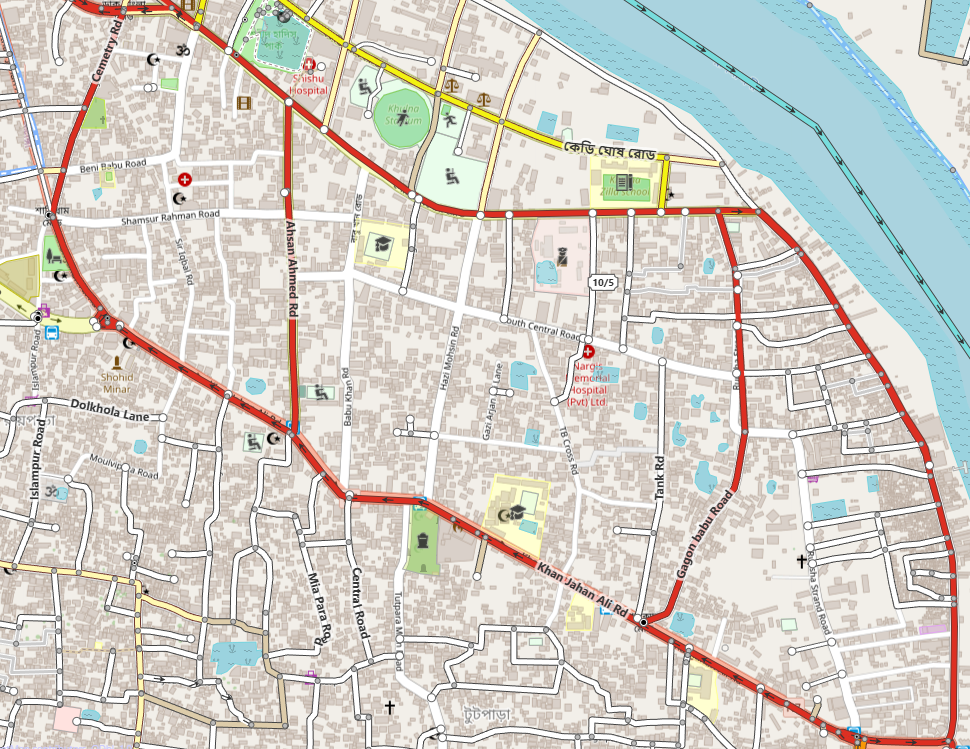
\includegraphics[width=\linewidth]{Khulna_Highlighted_OSM.png}
    \caption{}
  \end{subfigure}
  \hfill
  \begin{subfigure}[b]{0.48\columnwidth}
    \centering
    
\includegraphics[width=\linewidth]{SUMO_custom_road_network.png}
    \caption{}
  \end{subfigure}
  \caption{(a) A particular region's map of Khulna city from Open
           Street Map. (b) Simulated road (custom) network of Khulna
           city in SUMO, consisting of 11 directed edges (E0--E10)
           with 8 bidirectional routes and traffic-light-controlled
           intersections (red dots indicate junction nodes).}
  \label{fig:maps}
\end{figure}

\subsection{Heterogeneous EV Fleet}

To model Khulna's real Electric Vehicle ecosystem, three vehicle
classes with different battery configured: Easy Bikes(34 types),
Electric Rickshaws(33 types), Electric Vans(33 types). Total 100
continuous flows across the network. From 2 to 81 vehicles per
hour-launce vehicle through the 600 seconds simulation. Each vehicle
has a SUMO battery device with specific values: 345 kg vehicle mass,
0.760 air drag coefficient, 0.0155 rolling drag, 81\% propulsion
efficiency, and 64\% recovery efficiency \cite{b20}. Table~\ref{tab:fleet}
summarizes the three vehicle fleet classes. Significantly, the easy
bikes carry 12,000 Wh batteries, whereas the e-rickshaws and e-vans
are equipped with smaller batteries with 5,760--7,200 Wh batteries.
This scenario reflectes the actual mixed-fleet composition deployed in
Khulna. During simulation vehicles enter with different initial SoC
levels(12.9\% - 43.2\%), that reflects realistic field conditions.

\begin{table}[htbp]
\caption{Heterogeneous EV Fleet Configuration}
\label{tab:fleet}
\begin{center}
\begin{tabular}{|l|c|c|c|}
\hline
\textbf{Vehicle Type} & \textbf{Count} & \textbf{Battery (Wh)} &
  \textbf{\begin{tabular}[c]{@{}c@{}}Max Speed\\(m/s)\end{tabular}} \\
\hline
Easy Bike  & 34 & 12,000       & 8.33 \\
\hline
E-Rickshaw & 33 & 5,760--7,200 & 6.94 \\
\hline
E-Van      & 33 & 5,760--7,200 & 5.56 \\
\hline
\end{tabular}
\end{center}
\end{table}

\subsection{Charging Station Infrastructure}

10 charging stations are implanted as simulation parking areas over
2-way, 5-road corridors. Each of them has separate charging sub areas
and waiting sub areas. The charging sub areas have SUMO charging device
parameters like-charging power, efficiency of charging. They enable
local SUMO battery rechargeable. Table~\ref{tab:stations} explains
detailed configuration. Here the total system capacity is 62 charging
slots and 49-waiting slots. Station power rating range is : 25-50 kW
with 95\% efficiency.

\begin{table}[htbp]
\caption{Charging Station Configuration}
\label{tab:stations}
\begin{center}
\begin{tabular}{|l|c|c|c|c|}
\hline
\textbf{Station} &
  \textbf{\begin{tabular}[c]{@{}c@{}}Chg.\\Slots\end{tabular}} &
  \textbf{\begin{tabular}[c]{@{}c@{}}Wait.\\Slots\end{tabular}} &
  \textbf{\begin{tabular}[c]{@{}c@{}}Power\\(kW)\end{tabular}} &
  \textbf{Eff.} \\
\hline
pa\_1 (fwd) & 4  & 3 & 25    & 95\% \\
\hline
pa\_1\_rev  & 4  & 3 & 25    & 95\% \\
\hline
pa\_3 (fwd) & 5  & 4 & 30    & 95\% \\
\hline
pa\_3\_rev  & 8  & 6 & 40    & 95\% \\
\hline
pa\_5 (fwd) & 4  & 3 & 25    & 95\% \\
\hline
pa\_5\_rev  & 4  & 3 & 25    & 95\% \\
\hline
pa\_7 (fwd) & 6  & 5 & 35    & 95\% \\
\hline
pa\_7\_rev  & 6  & 5 & 35    & 95\% \\
\hline
pa\_8 (fwd) & 5  & 3 & 50    & 95\% \\
\hline
pa\_8\_rev  & 10 & 6 & 50    & 95\% \\
\hline
\textbf{Total} & \textbf{62} & \textbf{49} & 25--50 & 95\% \\
\hline
\end{tabular}
\end{center}
\end{table}

\subsection{TraCI Communication Layer}

TraCI gives a socket based API. It interacts with SUMO and Python. In
every integer second, the controller gathers battery parameters
(\texttt{device.battery.chargeLevel},
\texttt{device.battery.capacity},
\texttt{device.battery.totalEnergyConsumed}), vehicle location, speed,
current road ID, lane ID and stop status. It uses
\texttt{traci.simulation.findRoute()} to evaluate topological
reachability. This is an important step for directional
constraints---and \texttt{traci.lane.getShape()} to calculate Euclidean
station distances. Where a route change is possible and the vehicle's
SoC drops below the threshold value of 30\% warning. The controller
reroutes the vehicle to its assigned parking area(used as charging area
here) by calling \texttt{traci.vehicle.setRoute()} and
\texttt{traci.vehicle.setParkingAreaStop()}.

\subsection{Data Logging Module}

Each recommendation event is logged as 28 attribute CSV record:-
timestep, vehicle-type, current edge, lane, speed, SoC, battery
capacity, priority level and full metadata (ID, distance, power rating,
charging/waiting availability, occupancy rate) for both the nearest,
2nd nearest stations, plus textual reasoning string of the recommended
station. 1,169 recommendation events are generated in the simulation.
Moreover a vehicle-centric dataset contains 33,721 timestep vehicle
records with system level features. It includes total active vehicles,
charging vehicles, average SoC, system power demand, and per-vehicle
status and metrics.

%=======================================================
\section{Charging Recommendation Model}
%=======================================================

\subsection{Multi-Criteria Scoring Formulation}

At simulation time t, for a vehicle v requiring charging, the proposed
station-$S^{*}$ reduces a composite score over the set of N=10
available stations:

\begin{equation}
  S^{*} = \arg\min_{i}\;\bigl(w_1 D_i + w_2 Q_i + w_3 L_i\bigr)
  \label{eq:score}
\end{equation}

Where, $D_i$ = Euclidean distance from vehicle v to station $s_i$ (m),
$Q_i$ = number of vehicles currently in the waiting queue at $s_i$, and
$L_i$ = instant charging power load at $s_i$ (kW). Weighting factors
$w_1$ = 0.5, $w_2$ = 0.3, $w_3$ = 0.2 were set to prioritise proximity
while moderating congestion and load effects. Rankings are calculated
using Euclidean distance for computational efficiency at every 1 second
polling interval. The top two candidates (closest and second-closest).
Then go through the decision logic below.

\subsection{SoC Priority Classification}

Every recommendation event is tagged with one of 3 priority levels
based on the vehicle's current SoC: CRITICAL (SoC $<$ 20\%), HIGH
(20\% $\leq$ SoC $<$ 30\%), and MEDIUM (30\% $\leq$ SoC $<$ 50\%).
Priority-level tagging serves a significant purpose. It controls the
urgency of console alerts during simulation (CRITICAL and HIGH events
trigger verbose output).
\begin{itemize}
  \item \textbf{CRITICAL} (SoC $<$ 20\%): immediate action required
        --- risk of battery depletion in transit.
  \item \textbf{HIGH} (20\% $\leq$ SoC $<$ 30\%): urgent --- vehicle
        should charge at the next available opportunity.
  \item \textbf{MEDIUM} (30\% $\leq$ SoC $<$ 50\%): proactive
        recommendation --- vehicle can reach the station comfortably.
\end{itemize}

\subsection{Directional Constraint and Advisory Mode}

A notable innovation of this framework is SUMO's explicit handling of
directional routing constraints. In Khulna, easy bikes and e-rickshaws
operate on specific corridor routes. SUMO enforces one-way lane
assignments and cannot teleport vehicles to the opposite end. As a
result, the framework operates in two modes:

\textbf{Rerouting Mode}: When, {traci.simulation.findRoute()} -
returns a valid directed path from the vehicle's current end to the
target station end, with a positive route length, the framework calls
\texttt{setRoute()} and \texttt{setParkingAreaStop()} to redirect the
vehicle. A return route to the vehicle's original destination is added
if possible.

\textbf{Advisory Mode}: When no valid guided path exists, because of
the target station is at an unreachable distance from the vehicle's
recent running-structure, the framework logs the best scoring station
as suggested recommendation. It preserves simulation integrity and
produces useful data for real-world notification systems.

\subsection{Four-Rule Decision Logic}

Given the nearest station $s_1$ and second nearest station $s_2$. The
recommendation algorithm applies the following rules sequentially:
\begin{enumerate}
  \item \textbf{Rule 1}: If $s_1$ has a free charging slot $\rightarrow$
        recommend $s_1$ (Rerouting Mode if path exists).
  \item \textbf{Rule 2}: If $s_1$ is full for charging but $s_2$ has a
        free charging slot $\rightarrow$ recommend $s_2$.
  \item \textbf{Rule 3}: If $s_2$ also lacks charging slots but $s_2$
        has waiting capacity $\rightarrow$ recommend $s_2$ (waiting queue).
  \item \textbf{Rule 4}: If both $s_1$ and $s_2$ are fully saturated
        $\rightarrow$ recommend $s_1$ (Advisory Mode, flag for retry).
\end{enumerate}

A 30 second cooldown per vehicle prevents recommendation changes. Queue
management uses FIFO propagation:- when a charging vehicle leaves, the
next waiting vehicle will automatically promoted to a charging slot via
\texttt{traci.vehicle.resume()} and new \texttt{setParkingAreaStop()}
call. That maintains orderly slot throughput without outside
interference.

%=======================================================
\section{Simulation Setup and Parameters}
%=======================================================

Table~\ref{tab:params} summarizes the complete simulation parameter
set. \texttt{Test1.sumocfg} (SUMO configuration) specifies the road
network (\texttt{Test1\_with\_TLS.net.xml}), vehicle flows
(\texttt{Test1.rou.xml}) and charging infrastructure
(\texttt{Test1.chargingstations.add.xml}). Battery output, charging
station output, trip information and summary statistics are collected
via SUMO's native output facility. The Python controller
(\texttt{charging\_recommendation}) connects through TraCI, iterates in
1-second integer steps, and exports recommendations datasets to
timestamped CSV files after simulation completion at t = 600 seconds.

\begin{table}[htbp]
\caption{Key Simulation Parameters}
\label{tab:params}
\begin{center}
\begin{tabular}{|l|l|}
\hline
\textbf{Parameter} & \textbf{Value} \\
\hline
Simulator                         & SUMO (Eclipse) \\
\hline
Interface                         & TraCI (Python 3.x) \\
\hline
Simulation duration               & 600 s \\
\hline
Time step resolution              & 0.1 s \\
\hline
Number of vehicle flows           & 100 \\
\hline
Vehicle classes                   & Easy Bike, E-Rickshaw, E-Van \\
\hline
Number of routes                  & 8 (4 fwd + 4 rev) \\
\hline
Network edges                     & 11 directed \\
\hline
Charging stations                 & 10 bidirectional \\
\hline
Total charging slots              & 62 \\
\hline
Total waiting slots               & 49 \\
\hline
Charging power range              & 25--50 kW \\
\hline
Charging efficiency               & 95\% \cite{b21}\\
\hline
SoC trigger threshold             & 50\% \\
\hline
CRITICAL priority                 & SoC $<$ 20\% \\
\hline
HIGH priority                     & 20\% $\leq$ SoC $<$ 30\% \\
\hline
Recommendation cooldown           & 30 s \\
\hline
Scoring weights ($w_1, w_2, w_3$) & 0.5, 0.3, 0.2 \\
\hline
\end{tabular}
\end{center}
\end{table}

%=======================================================
\section{Results and Discussion}
%=======================================================

\subsection{System Load and Charging Statistics}

The simulation ended at 600 s. It generates 33,721 vehicle centric
records(one vehicle per second) and 1,169 charging recommendation
events. The system recorded a peak instant charging power of 1,370 kW
with 40 vehicles charging concurrently. That reflects near saturation
of the 62 available charging areas during peak demand time. Across the
simulation the average charging power was 963.7 kW, the total energy
consumption for charging was 127.5 kWh. These load metrics highlights
that there is an important charging demand on the network. It makes
intelligent station selection essential to prevent local transformer
overload.

\subsection{Recommendation Volume and Priority Distribution}

Table~\ref{tab:priority} shows the priority level breakdown of the
1,169 recommendation events. HIGH-priority events (SoC 20\%--30\%)
dominated at 42.7\%, followed by MEDIUM (34.6\%) and CRITICAL (22.7\%).
The average SoC at the time of recommendation was 27.7\%
($\sigma$ = 8.5\%), with a minimum of 12.0\% and a maximum of 46.5\%.
It ensures that the 50\% trigger activates recommendations with
sufficient battery margin. The average Euclidean distance to the
nearest station at the time of recommendation was 84.3 m
($\sigma$ = 62.0 m, min = 0.5 m, max = 256.6 m). It is indicating
adequate station density for the modelled fleet.

\begin{table}[htbp]
\caption{Recommendation Priority Distribution}
\label{tab:priority}
\begin{center}
\begin{tabular}{|l|c|c|c|}
\hline
\textbf{Priority} & \textbf{SoC Range} & \textbf{Events} & \textbf{Pct.} \\
\hline
CRITICAL & $<$20\%      & 265 & 22.7\% \\
\hline
HIGH     & 20\%--30\%   & 499 & 42.7\% \\
\hline
MEDIUM   & 30\%--50\%   & 405 & 34.6\% \\
\hline
\textbf{Total} & ---    & \textbf{1,169} & \textbf{100\%} \\
\hline
\end{tabular}
\end{center}
\end{table}

\subsection{Recommendation Outcome Analysis}

Table~\ref{tab:outcomes} shows the distribution of the results of
recommendations. The main result --- when charging slots were available,
59.0\% (689 events)---was routing to the nearest station. In 24.1\% of
cases (282 events), the nearest station was fully occupied and vehicles
were successfully directed to the second nearest station with available
capacity. It is demonstrating genuine load diversion. Where both
stations were saturated, Waiting slot overflow management handled 7.7\%
(90 events), while 9.2\% (108 events) triggered Advisory Mode.

\begin{table}[htbp]
\caption{Recommendation Outcome Analysis}
\label{tab:outcomes}
\begin{center}
\begin{tabular}{|l|c|c|}
\hline
\textbf{Outcome} & \textbf{Events} & \textbf{Pct.} \\
\hline
Nearest station (slot available)  & 689 & 59.0\% \\
\hline
2nd nearest (nearest full)        & 282 & 24.1\% \\
\hline
Waiting slot overflow             & 90  &  7.7\% \\
\hline
Advisory Mode (both saturated)    & 108 &  9.2\% \\
\hline
\textbf{Total}                    & \textbf{1,169} & \textbf{100\%} \\
\hline
\end{tabular}
\end{center}
\end{table}

\subsection{Station Utilisation Distribution}

Station pa\_8 received the highest recommendation share (32.4\% of all
events). Which reflects its large slot capacity (5 charging + 3 waiting
forward, 10 + 6 reverse) and power rating up to 50 kW combined with a
central network position. Stations pa\_7 and pa\_3\_rev came in second
and third with 14.7\% and 14.0\% respectively. Significantly, all ten
stations received at least 1.5\% of recommendations, confirming that
the multi-criteria scoring model \cite{b7, b12} widely distributes demand.

\subsection{Comparative Evaluation: Proposed vs. Nearest-Only Baseline}

To measure the benefit of the structure, we define a nearest-only
baseline that always recommends the Euclidean nearest station without
considering occupancy, queue, or load. Table~\ref{tab:comparison} shows
4-performance metrics computed from the 1,169-event dataset.

\begin{table}[htbp]
\caption{Performance Comparison: Proposed vs. Nearest-Only Baseline}
\label{tab:comparison}
\begin{center}
\begin{tabular}{|l|c|c|}
\hline
\textbf{Metric} & \textbf{Proposed} & \textbf{Baseline} \\
\hline
Feasible Rec.\ Rate (FRR)       & 90.1\% & 66.0\% \\
\hline
Congestion Avoid.\ Rate (CAR)   & 37.1\% &  0.0\% \\
\hline
Hi-Priority Smart Dec.\ (HPSDR) & 27.9\% &  0.0\% \\
\hline
Avg.\ Distance (m)              & 100.1  &  84.3  \\
\hline
\end{tabular}
\end{center}
\end{table}

The following subsections explain each metric in depth - its definition,
calculation method, numerical values and significance in this work.

\subsubsection{Feasible Recommendation Rate (FRR)} FRR is the fraction of all recommendation events,
in which the station recommended by the algorithm had at least one free
charging slot available at the time of recommendation. A recommendation
is ``feasible'' if a vehicle dispatched to the station can immediately
begin charging without waiting for a slot to become vacant.

\textbf{Calculation Formula}:
\begin{equation}
  \text{FRR} =
    \frac{N_{\text{rec.\ station} \geq 1 \text{ free slot}}}
         {N_{\text{total events}}}
    \times 100\%
  \label{eq:frr}
\end{equation}

For the proposed framework, the feasible events are those resolved by
Rule 1 (689 events, nearest with free slot) plus Rule 2 (282 events,
2nd nearest with free slot) = 971 feasible events out of 1,169 total.
\begin{equation}
  \text{FRR (Proposed)} = \frac{971}{1{,}169} \times 100\% \approx 90.1\%
  \label{eq:frr_prop}
\end{equation}

For the baseline, the nearest station is feasible only in those 771
events (66.0\% of 1,169) in which the nearest station happened to have
a free slot regardless of diversion. The baseline makes no attempt to
check or redirect to a better option.

\textbf{Interpretation}: An FRR of 90.1\% means that out of every 100
recommendation events, 90 result in the vehicle being directed to a
station where it can plug in immediately. The 24.0 percentage-point
improvement over the baseline quantifies the concrete benefit of
occupancy-aware selection: vehicles are far less likely to arrive at a
full station, waste time waiting, or drain their already-depleted
battery in further searching.

\subsubsection{Congestion Avoidance Rate (CAR)} CAR measures the proportion of all recommendation
events in which the proposed framework successfully diverted a vehicle
away from a congested (fully occupied) nearest station to an alternative
station with available capacity. It directly quantifies the
load-balancing effectiveness of the recommendation engine.

\textbf{Calculation Formula}:
\begin{equation}
  \text{CAR} =
    \frac{N_{\text{nearest full \& alt.\ with free slots}}}
         {N_{\text{total events}}}
    \times 100\%
  \label{eq:car}
\end{equation}

This corresponds exactly to Rule 2 events: 282 cases in which the
nearest station was fully occupied but the second-nearest had capacity.
The baseline, which blindly recommends the nearest station, contributes
0 such diversions.
\begin{equation}
  \text{CAR (Proposed)} = \frac{282}{1{,}169} \times 100\% = 37.1\%
  \label{eq:car_prop}
\end{equation}
\begin{equation}
  \text{CAR (Baseline)} = 0.0\%
  \label{eq:car_base}
\end{equation}

\textbf{Interpretation}: A CAR of 37.1\% means that more than one in
three charging events that would have overloaded a popular station are
instead redistributed to a less congested alternative. In grid terms,
this translates directly to reduced transformer peak loading, lower risk
of thermal stress, and more uniform utilisation of the installed
charging infrastructure. The baseline's CAR of 0\% confirms that
proximity-only dispatching cannot achieve any congestion relief by
design.

\subsubsection{High-Priority Smart Decision Rate (HPSDR)}
 HPSDR measures the proportion of CRITICAL
(SoC $<$ 20\%) and HIGH (20\% $\leq$ SoC $<$ 30\%) priority
recommendation events --- those carrying the highest battery urgency ---
in which the framework successfully diverted the vehicle to the
second-nearest station because the nearest station lacked available
charging slots. It captures intelligent decision-making precisely when
the stakes are highest: when battery depletion in transit is a realistic
risk.

\textbf{Calculation Formula}:
\begin{equation}
  \text{HPSDR} =
    \frac{N_{\text{CRIT+HIGH: chose 2nd over congested 1st}}}
         {N_{\text{total events}}}
    \times 100\%
  \label{eq:hpsdr}
\end{equation}

CRITICAL events: 265; HIGH events: 499; combined = 764 high-urgency
events out of 1,169 total (65.4\%). Of these, the framework
successfully diverted to the second-nearest station (Rule 2 applied
during CRITICAL/HIGH events) in 27.9\% of all events = 326 events.
\begin{equation}
  \text{HPSDR (Proposed)} = \frac{326}{1{,}169} \times 100\% = 27.9\%
  \label{eq:hpsdr_prop}
\end{equation}
\begin{equation}
  \text{HPSDR (Baseline)} = 0.0\%
  \label{eq:hpsdr_base}
\end{equation}

\textbf{Interpretation}: An HPSDR of 27.9\% demonstrates that the
framework does not apply a blanket nearest-station rule even under
battery urgency --- it actively reasons about availability and routes
critically depleted vehicles to the best accessible station. The 27.9
percentage-point advantage over the baseline is particularly significant
in the Khulna context, where running out of charge mid-route leaves an
Easy Bike or E-Rickshaw stranded, blocking traffic and causing immediate
income loss for the driver. The baseline achieves HPSDR = 0\% because
it has no mechanism to deviate from the nearest station regardless of
urgency level.

\subsubsection{Average Distance to Recommended Station}: This metric reports the mean Euclidean
straight-line distance (in metres) from a vehicle's position at the
moment of recommendation to the station it is recommended to visit. It
serves as the primary cost metric to assess the trade-off incurred by
congestion-aware routing: redirecting vehicles to alternative stations
necessarily increases travel distance.


\textbf{Calculation Formula}:
\begin{equation}
  \overline{d} =
    \frac{1}{N}\sum_{i=1}^{N}
      d_{\text{Eucl.}}\!\bigl(\mathrm{pos}_{i},\;
                               s_{i,\,\text{rec}}\bigr)
  \label{eq:avgdist}
\end{equation}

where N = 1,169 total recommendation events, $\mathrm{pos}_{i}$ is the
vehicle's geographic coordinates at event i, and
$s_{i,\,\text{rec}}$ is the centre coordinates of the recommended
station. Euclidean distance is computed using
\texttt{traci.lane.getShape()} coordinate data polled at each integer
second.
\begin{align}
  \overline{d}_{\,\text{Baseline}} &= 84.3\;\text{m}
    \quad\text{(always the nearest station by definition)}
    \label{eq:dist_base}\\
  \overline{d}_{\,\text{Proposed}} &= 100.1\;\text{m}
    \quad\text{(can be the 2nd nearest)}
    \label{eq:dist_prop}
\end{align}

\textbf{Interpretation}: The proposed framework asks vehicles to travel,
on average, 15.8 m further than the nearest station. This is the
accepted cost of avoiding congested stations. To contextualise this
trade-off, consider that the average SoC at recommendation time is
27.7\% and the minimum battery capacity is 5,760 Wh. Even at an average
propulsion power of ${\sim}$1.5 kW and a speed of 10 m/s, the
additional 15.8 m adds less than 2 seconds of travel time and consumes
a negligible energy increment well within the available battery margin.
The trade-off is therefore operationally inconsequential while the gains
in FRR (+24.0 pp), CAR (+37.1 pp), and HPSDR (+27.9 pp) are
substantial.

\subsubsection{Summary Comparison and Interpretation}

Table~\ref{tab:comparison} consolidates all four metrics. The proposed
multi-criteria framework outperforms the nearest-only baseline on every
effectiveness dimension while incurring a trivially small distance
penalty. The combined picture is as follows:

\textbf{FRR (90.1\% vs 66.0\%)}: 9 in 10 recommended stations have
free slots immediately, versus only 2 in 3 under naive routing. This
reduces wasteful station-to-station re-querying by vehicles already at
low SoC.

\textbf{CAR (37.1\% vs 0.0\%)}: The framework actively load-balances
by redirecting more than a third of all events away from congested hubs
to underutilised alternatives, reducing transformer peak stress and
prolonging infrastructure lifetime.

\textbf{HPSDR (27.9\% vs 0.0\%)}: Even the most critically
battery-depleted vehicles receive superior routing --- the framework
exercises its highest priority triage precisely when failures are most
costly in the real world.

\textbf{Avg. Distance (+15.8 m)}: The marginal extra travel introduced
by smarter routing is 15.8 m --- less than 2 vehicle lengths --- and is
operationally negligible relative to the energy and time benefits
delivered.

\subsection{Limitations and Future Work}

The 600-second simulation window incorporates a simple network. Full
scale deployment requires GPS trace calibrated OD matrices and different
charging profiles from field surveys. Advisory Mode (9.2\% of
occurrences) can be reduced by increasing station density or adding a
3rd nearest candidate. Future work will integrate dynamic electricity
pricing and renewable energy at station nodes.

%=======================================================
\section{Implications for Bangladesh}
%=======================================================

The 37.1\% Congestion Avoidance Rate suggests that approximately one in
three charging events that would otherwise overload a popular station
can be redistributed. This can reduce peak transformer loading and
increasing equipment lifetime. The resulting datasets (33,721
vehicle-centric + 1,169 recommendation events) accurately provides the
feature space separated valued columns.

The per station recommendation distribution reveals that pa\_8 and
pa\_7 corridors absorb inconsistent demand- which directly actionable
information for capacity increasing. The open SUMO+Python architecture
enables urban or city planners to test alternative station placements
by modifying the XML configuration without specialised optimization
skills.

%=======================================================
\section{Conclusion}
%=======================================================

This paper shows a SUMO+TraCI simulation-based charging station
recommendation framework for heterogeneous EV fleet in Khulna city. A
100 flow simulation through 3- vehicle classes with varying battery
capacities (12,000 Wh for Easy Bikes; 5,760--7,200 Wh for E-Rickshaws
and E-Vans), eight routes and ten bidirectional stations generated 1,169
recommendation events over 600 seconds. Also depicts the record of peak
charging power of 1,370 kW with 40 vehicles simultaneously charging and
consuming 127.5 kWh total energy.

The main contributions are: (1) a physics-calibrated SUMO fleet model
with different battery configurations across three vehicle classes;
(2) a multi-criteria recommendation algorithm with Advisory duality;
(3) comparative evaluation demonstrating +24.0 pp potential
Recommendation Rate, +37.1 pp Congestion Avoidance Rate, and +27.9 pp
High-Priority Smart Decision Rate versus a nearest-only baseline; and
(4) two complementary datasets (33,721 vehicle-centric records +
1,169 recommendation events).

Future work will be expanded to include GPS trace calibration of the
full road graph of Khulna, dynamic pricing, model renewable energy at
stations and evaluate demand-response schedules consistent with
Bangladesh's National Energy Policy.

%=======================================================
\begin{thebibliography}{00}

\bibitem{b1}
M.~A. Rahman, S.~Islam, and A.~H. Khan, ``Electric vehicle adoption
trends in Bangladesh: Opportunities and challenges,'' \textit{IEEE
Access}, vol.~9, pp.~145632--145645, 2021.

\bibitem{b2}
D.~Wang, J.~Guan, T.~Wu, G.~Zheng, and Y.~Hu, ``Intelligent charging
station selection for electric vehicles using multi-objective
optimization,'' \textit{IEEE Trans. Intell. Transport. Syst.}, vol.~23,
no.~8, pp.~11234--11245, Aug. 2022.

\bibitem{b3}
C.~Pascual, \textit{Global EV Outlook 2022}. Paris, France: IEA, 2022.
[Online]. Available:
\url{https://www.iea.org/reports/global-ev-outlook-2022}

\bibitem{b4}
S.~Chen, Y.~Tong, and W.~Hu, ``TraCI-based real-time traffic control
in SUMO simulation,'' \textit{J. Traffic Transport. Eng.}, vol.~7,
no.~3, pp.~315--328, 2020.

\bibitem{b5}
X.~Zhang, Q.~Wang, and L.~Li, ``Load balancing strategies for electric
vehicle charging stations using reinforcement learning,'' \textit{IEEE
Trans. Smart Grid}, vol.~13, no.~4, pp.~3124--3135, Jul. 2022.

\bibitem{b6}
A.~Hussain, V.~H. Bui, and H.~M. Kim, ``A multi-criteria
decision-making approach for electric vehicle charging station location
selection,'' \textit{Energies}, vol.~13, no.~23, p.~6322, 2020.

\bibitem{b7}
M.~R. Islam, H.~Lu, J.~Hossain, and L.~Li, ``A review on energy
management strategies for electric vehicles in developing countries: A
case study of Bangladesh,'' \textit{Renew. Sustain. Energy Rev.},
vol.~141, p.~110803, 2021.

\bibitem{b8}
J.~Siddiqui, U.~Ahmed, A.~Amin, T.~Alharbi, A.~Alharbi, I.~Aziz,
A.~R. Khan, and A.~Mahmood, ``Electric vehicle charging station load
forecasting with an integrated DeepBoost approach,'' \textit{Alexandria
Eng.\ J.}, vol.~116, pp.~331--341, Jan. 2025.

\bibitem{b9}
P.~A. Lopez \textit{et al.}, ``Microscopic traffic simulation using
SUMO,'' in \textit{Proc. 21st Int. Conf. Intell. Transport. Syst.
(ITSC)}, Maui, HI, USA, 2018, pp.~2575--2582.

\bibitem{b10}
``Battery-run vehicles add to Khulna's power woes,'' \textit{The Daily
Star}, Sep. 30, 2022. [Online]. Available:
\url{https://www.thedailystar.net/news/bangladesh/news/battery-run-vehicles-add-khulnas-power-woes-3132111}

\bibitem{b11}
``High penetration of electric autorickshaw on national power system
and barriers against the adoption of solar energy: A case study in
Bangladesh,'' \textit{Energy Nexus}, 2023. [Online]. Available:
\url{https://www.sciencedirect.com/science/article/pii/S2666790823000423}

\bibitem{b12}
``Evaluating the socio-economic and environmental impact of battery
operated auto rickshaw in Khulna city,'' in \textit{Proc. Int. Conf.
Civil Eng. Sustainable Dev. (ICCESD)}, KUET, 2018. [Online]. Available:
\url{https://iccesd.kuet.ac.bd/2018/Papers/r_p4650.pdf}

\bibitem{b13}
``Dynamic load balancing for EV charging stations using reinforcement
learning and demand prediction,'' \textit{ResearchGate}, 2024.
[Online]. Available:
\url{https://www.researchgate.net/publication/389714334}

\bibitem{b14}
``A multicriteria GIS-based decision-making approach for locating
electric vehicle charging stations,'' \textit{ResearchGate}, 2022.
[Online]. Available:
\url{https://www.researchgate.net/publication/362470657}

\bibitem{b15}
``Adaptive traffic signaling control using SUMO simulator,''
\textit{IJISRT}, Jan. 2025. [Online]. Available:
\url{https://www.ijisrt.com/assets/upload/files/IJISRT25JAN158.pdf}

\bibitem{b16}
``Relentless load shedding plagues Khulna, Barishal residents,''
\textit{TBS News}. [Online]. Available:
\url{https://www.tbsnews.net/bangladesh/energy/relentless-load-shedding-plagues-khulna-barishal-residents-981976}

\bibitem{b17}
``Carrying full passengers in easy bikes can ease traffic, save power:
Research,'' \textit{BSS News}, Sep. 14, 2025. [Online]. Available:
\url{https://www.bssnews.net/others/311737}

\bibitem{b18}
International Energy Agency (IEA), \textit{Global EV Outlook 2025}.
Paris, France: IEA, 2025. [Online]. Available:
\url{https://www.iea.org/reports/global-ev-outlook-2025}

\bibitem{b19}
``Multi-objective optimization strategy for intelligent charging and
discharging station of electric vehicles in the distribution network,''
\textit{IEEE Access}, 2021. [Online]. Available:
\url{https://ieeexplore.ieee.org/document/9511077}

\bibitem{b20}
``A review on energy management systems in battery electric vehicles,''
\textit{ResearchGate}, 2023. [Online]. Available:
\url{https://www.researchgate.net/publication/400355371}

\bibitem{b21}
West Zone Power Distribution Company Limited (WZPDCL), \textit{Khulna
Division Distribution Report}, 2023. [Online]. Available:
\url{https://file-khulna.portal.gov.bd/uploads/d07c3114-12a6-4ebe-8fa0-460e27018e82/671/5a0/75b/6715a075bfbf0518800500.pdf}


\end{thebibliography}

\end{document}